
% Make first version of the introduction section consist of four
% paragraphs. Add paragraphs later if needed.

\chapter{Introduction}
\label{ch:introduction}

% usually 2-4 pages, you can use ``I'' or "We'' when you
% describe what you have done


% 1. Introduction to the problem and problem statement:
% why is the work needed/done, how will ``the world'' benefit from it.
% everybody with some education should be able to read this part
% and understand that the thesis is useful
% you can use sections for these parts\section{Motivation and Problem Statement}

% 2. how do you attack the problem including the method (analysis, 
% experimentation etc)

% 3. other possible approaches or solutions

% 4. describe your solution and the summarize the main results,
%    if possible the research contributions

% 5: Thesis structure: outline of rest of thesis

\com{
    
    This\todo{The first paragraph after a heading is not indented, all of the
      subsequent paragraphs have their first line indented.} chapter describes the
    specific problem that this thesis addresses, the context of the problem, the
    goals of this thesis project, and outlines the structure of the thesis.\\
    
    \todo[inline]{Give a general introduction to the area. (Remember to use appropriate references in this and all other sections.)}
    
    at \SI{20}{cm}.
}

\noindent 
Autonomous systems development has improved consistently in the later period, providing improvements to every day life.
These systems are able to autonomously execute their tasks without human interaction and to adapt to dynamic settings.
On the field of robotics, their support is relevant when tasks are repetitive and the human presence is not necessary.
In the specific case of mobile robotics, autonomous navigation is required and those systems can achieve it using knowledge of their pose and surroundings.

The pose of a mobile robot can be estimated using sensors which provide measurements of their environment.
Multiple types of sensors are available, with difference in frequency, phenomenon captured, and reliability.
Heterogeneous sensors provide measurements which need to be properly fused together to improve the individual knowledge that they provide.

The awareness and the precision related to the position in the working environment changes with respect to each application.
The first autonomous mobile robots available to the consumers were the indoor cleaning robots, where simple collision detection is enough to wander in the indoor environment.
A more recent consumer application of such robots is the \gls{ALM}, which works in the complicated outdoor setting.

This master thesis investigates how to improve the performance of an \gls{ALM} providing localisation and mapping features using a set of heterogeneous sensor directly mounted on it.
It will focus on the implementation and analysis of a module based on the fusion of the measurements provided by different configurations of those sensors to remove the need of relying on external infrastructure. 
%An overview of the best settings for a precise localisation is provided
%Different configurations of sensors and techniques to fuse their measurements are investigated to provide an overview of the best setting to improve the localisation performance.
Finally, their configurations are investigated through multiple experiments, and drawbacks and improvements of each sensor are analysed.


\section{Background}
\label{sec:background}
%Present the background for the area. Set the context for your project – so that your reader can understand both your project and this thesis. (Give detailed background information in Chapter 2 - together with related work.)
%Sometimes it is useful to insert a system diagram here so that the reader knows what are the different elements and their relationship to each other. 
%This also introduces the names/terms/… that you are going to use throughout your thesis (be consistent). This figure will also help you later delimit what you are going to do and what others have done or will do.


\noindent \gls{ALM}s mow the lawn using a random walk coverage approach~\cite{karol_ardic_conditional_2016}, i.e. they move in a random direction until they detect a specific underground wire or until they collide with an object.
They will then rotate towards another direction and keep on going with this behavior. 
To do so, they rely in a minimal set of sensors to achieve their goals in dynamic outdoor environments.

Boundary wires are laid underground to provide the outer limits of the lawn working area, and some guide wires are used to aid the mobile robot with more complex tasks that the random behaviour will not be able to address, such as the autonomous return to the charging base and the navigation through narrow passages. 
These wires have a proprietary electrical current signal passing through and the mobile robot is able to detect it using three different magnetometer sensors, one positioned in the center front and the other two placed on each side.
Through the analysis of the magnetic field direction and pulses, the lawn mower is able to understand if the wire defines a boundary or if it provides a guide to go towards another area of the lawn or back to the charging base.
However, these external wires require regular maintenance which could be avoided with a more sophisticated model.

Additionally, the \gls{ALM}s implement collision sensors, located near the rear wheels.
When the mobile robot bumps into any firm object from the front, it will trigger push sensors situated on the chassis.
It has been used to react in case of collision with unexpected objects, but eventually it could be used to map the environment with those objects and avoid them systematically.

In more sophisticated and recent models, additional frontal ultrasonic range sensors are installed to slow down the mobile robot before potentially colliding with objects in its trajectory.

The most advanced models also include \Glspl{GNSS} receivers to keep track of the global robot position, for theft protection and lawn monitoring purposes.
However, it is not precise enough on its own to provide real time localisation information for it to be used for navigation purposed by the \gls{ALM}, but it can be used to detect that a particular side of the lawn has not been mowed in a while.% using the random walk coverage approach.

This configuration does not require them to understand their position on the world, as they just use a reactive architecture defined by a random behaviour motion pattern without any understanding of their surroundings~\cite{wooldridge_agent_1995}.
These robots are situated, i.e. they are not taking into account events of the past and they cannot foresee their future interactions with the environment  ~\cite{muller_1999}. 
As such, they are not able to plan ahead their path and they just react to perceptions of their surroundings.
They do not have a model of their world, and they do not need to update it in case of unexpected changes of their environment~\cite{wooldridge_agent_1995}. 
They are flexible and adaptive as they rely on the infrastructure manually installed for them~\cite{wahde2012introduction},  which however requires additional installation and maintenance.


\section{Problem}
\com{
Longer problem statement\\
If possible, end this section with a question as a problem statement.
}

\noindent 
The current method of autonomously mowing the lawn is not effective, since it is based on an external infrastructure to perform a reactive behaviour based on random walk coverage algorithm~\cite{karol_ardic_conditional_2016}, which cannot guarantee a complete coverage of the area.
%Random planning cannot guarantee a complete coverage, whereas, many deterministic techniques are not solely eligible for unstructured outdoor environments, since they highly suffer from wheel slippage or numerical drift. Besides, complete coverage techniques either demands high computational power or expensive sensor hardware.
This configuration for the \gls{ALM}s was given by constraints related to the low computational power available in the past.
Moreover, the recent progresses in the performance of embedded devices and sensors have made their navigation model obsolete, and as those components have also lowered their cost, their implementation is now feasible even for consumer products. 
The combined availability of more advanced devices and more computational power enables for the implementation of real time applications to improve the performances of these mobile robots. 


The performance of an \gls{ALM} can be improved with a more advanced perception and action system used to implement deterministic techniques of coverage planning.
The problem that needs to be solved is the development of a more precise localisation and mapping module, as with a better configuration, it would be possible to reach a more accurate understanding of the mobile robot pose inside a map of the lawn itself.
The \gls{ALM}, to perceive its surroundings and act accordingly, needs additional computational power  and sensors than the ones available in the current configurations.
An analysis of the best configuration of sensors, along with their measurements fusion, is needed to understand how to provide to costumers a more reliable product which needs no maintenance of the external infrastructure.
The issue is related to finding the most appropriate technique to fuse all these sensors' measures in a setting where every downside is compensated and every useful aspect of those sensors is exploited and highlighted,


An aspect that is worth investigating is related to the removal of the need of external infrastructure for localisation. 
Instead of relying to a vulnerable boundary wire, the implementation of such a system without installing additional and external devices on the lawn, and with a set of sensors built in the automower directly and removing the need for external infrastructure, will improve on multiple aspects and thus offer a more complete set of features for the users. 
Additionally, the removal of such a boundary wire or additional infrastructure will allow the automower to cover larger areas of custom configuration. Finally, the fused combination of given control commands and the whole set of sensors at disposal for this project has yet to be investigated in research, as usually fewer sensors are available. 


%\subsection{Scientific and engineering issues}
%The scientific relevance of this project is derived from the fact that outdoor localisation and mapping of dynamic environments are still far from reaching a reliable solution. 
%This work will aid in the handling of dynamical outdoor settings. 
%Since there are just few available devices able to mow the lawn without installing additional and external devices on the lawn, this work will investigate how it can be done using a set of sensors built in the automower directly and removing the need for external infrastructure. This work will provide valuable insights about this heterogeneous sensor fusion.



\section{Related Works}

\noindent 
The improvement of a robotic lawn mower is a recent research topic. It has emerged thanks to a set of research outcomes which have provided tools to increase the possible features that a automower can achieve.
Previous development of such mobile robots from scratch can be found in multiple reports.
They provide a complete analysis of all the components and a comprehensive view about the features to be provided on an \gls{ALM}.
The complete development of a fully featured mobile robot for golf course mowing, as part of a yearly robotics course, is detailed in~\cite{noauthor_groundsbot_nodate}.
A recent master thesis about the development robotic lawn mower with Visual SLAM and terrain classifier is described in~\cite{lukas_robotic_2020}.
A bachelor thesis regarding the prototyping of a mower using a camera and GPS in available in~ \cite{andersson_smart_2018}.
Both of these works did not manage to deliver on the desired outcomes. This is given mostly by the lack of time considering they had to also build the infrastructure of the mower.

Different approaches for localisation on a similar \gls{HRP} are described in~\cite{oden_localization_2017} using \gls{GPSRTK} external infrastrucTure and in~\cite{lensund_local_2018} using \gls{UWB} sensors on the mower.
In these cases however, there is the requirement for external devices to localise the \gls{ALM} and this aspect is not part of the scope of this thesis. 


\subsection{Competitor Analysis}

\noindent As this master thesis has been developed under the programme of EIT Digital\footnote{\url{https://masterschool.eitdigital.eu/}}, an analysis of the competitor will be performed to highlight the current state of the art at an industrial level for \gls{ALM}s which require no boundary wire installation, understanding their current implementations and evaluating possible improvements.

Toadi\footnote{\url{https://www.toadi.com/}} is a startup company based in Belgium which offers as only product an \gls{ALM} of the same name. It employs a single visual sensor system to provide the localisation features. It can mow an area of \SI{4800}{\meter\squared}.
Its installation is performed though a track and follow approach to determine the boundaries of the lawn, it has been in testing phase and it is available to the public from May 2021.

The LUNA platform from Inertial Systems\footnote{\url{https://inertialsense.com/autonomy/}} employs all the sensors listed above to provide a localisation and navigation module, which has been used for \gls{ALM}s. This platform was developed to enable engineers to directly embed autonomous capability into existing equipment avoiding the development of a localisation module, as it is detailed in this thesis.

Kingdom Technologies\footnote{\url{https://www.kingdom.garden/}} provide an \gls{ALM} at a monthly fee to commercial clients.
It employs sensor fusion techniques to merge several different sensors' measures to improve the positioning of the robot on a lawn that could reach an area of \SI{7500}{\meter\squared}.

Ambrogio L60 Elite S+\footnote{\url{https://www.ambrogiorobot.com/en/models/view/l60-elite-s}} requires no installation for areas up to \SI{400}{\meter\squared}.
It employs a grass sensor to detect the presence of grass under itself and it uses a specific robotic joint to recognise any holes or empty spaces. With these sensors it is able to navigate around a defined lawn using a reactive approach, but without the need for the boundary wire.

Different approaches which do not require the boundary wire installation but which still need some external infrastructures are the following.

Husvarna 550 EPOS\footnote{\url{https://www.husqvarna.com/us/products/robotic-lawn-mowers/models/automower-550-epos/}} is a new automower available for commercial customers which employs a \gls{GPSRTK} sensor to cover areas of \SI{5000}{\meter\squared}. It needs an external and expensive receiver to correct the \gls{GNSS} estimates of the robot and improve its localisation performances to just a few centimeters error.

iRobot Terra t7\footnote{\url{https://www.irobot.co.uk/Terra}} is the \gls{ALM} 
It relies on wireless navigation beacons installed on the garden to triangulate the position of the mower using their signals. However, the implementation of such technology has concerned the \gls{NRAO}, as the original intended frequency they used were disturbing the measurements of that organisation, and they had to change their beacons using \gls{UWB} signal technology. 

The currently developed \gls{ALM}s are still far from being mature and available to all customers.
For this reason, an analysis of the best configuration of sensors to improve on the localisation aspects without the need for an external installation is provided, as improved localisation performances of autonomous mobile robots are required.

Numerous related studies and implementations have been developed in similar topics to improve localisation features, and the analysis of an optimal configuration of sensors which require no external installations is still relevant to the best of the found knowledge.


\section{Research Goals}

\com{
State the purpose  of your thesis and the purpose of your degree project.

Describe who benefits and how they benefit if you achieve your goals. Include anticipated ethical, sustainability, social issues, etc. related to your project. (Return to these in your reflections in Section~\ref{sec:reflections}.)

State the goal/goals of this degree project.
 
This has been divided into the following three sub-goals:
\begin{enumerate}
\item Subgoal 1 \todo[inline, backgroundcolor=aqua]{för att tillfredsställa problemägaren – industrin?}
\item Subgoal 2\todo[inline, backgroundcolor=aqua]{för att tillfredsställa ingenjörssamfundet och vetenskapen – akademin) }
\item Subgoal 3\todo[inline, backgroundcolor=aqua]{eventuellt, för att uppfylla kursmålen – du som student}
\end{enumerate}

In addition to presenting the goal(s), you might also state what the deliverables and results of the project are. 
}

\noindent Autonomously mowing the lawn will help saving time and avoid human intervention as much as possible. The steps needed to improve current systems are related to a dynamic management of the boundary of the lawn, eliminating the need for a boundary wire and its related installation and maintenance.

The knowledge about position and orientation of the mobile robot with respect to a map enables for the application of more deliberative architectures~\cite{genesereth_logical_1987}.
With this architecture, the pose with respect to a map will allow the \gls{ALM} to make independent decisions and to plan its path to cover the lawn in a shorter amount of time, leaving a better pattern, avoiding unexpected objects, and saving energy and resources.
%The term `deliberative agent' seems to have derived from Genesereth's use of the term `deliberate agent' to mean a specific type of symbolic architecture [Genesereth and Nilsson, 1987].) We define a deliberative agent or agent architecture to be one that contains an explicitly represented, symbolic model of the world, and in which decisions (for example about what actions to perform) are made via logical (or at least pseudo-logical) reasoning, based on pattern matching and symbolic manipulation. ~\cite{genesereth_logical_1987}

The goal of this thesis is to provide an overview on how to develop a precise localisation module for an \gls{ALM}
An analysis about different configurations of sensors and about how to fuse their measures using sensor fusion filters is defined.
As end result, the \gls{ALM} will be able to operate in a specified environment without the need to intervene with the installation of additional infrastructure, but just with the addition of heterogeneous sensors installed directly on the mobile robot.

The focus of this degree project is the precise localisation inside a predefined given map to ensure that the automower stays inside the virtual boundaries defined.
Moreover, a map of the lawn is developed to allow for updates using collision events against unexpected object to provide a more dynamic view of the lawn.
%It will benefit both the industry of \gls{ALM} with the knowledge derived from this thesis, and the consumers will obtain a product which requires less maintenance.

The research questions to be evaluated are the following:
\begin{itemize}
    \item Providing an initial map and location of the automower in it, will the automower be able to stay within the given boundaries with a specified margin for error?
    \item Will the automower be able to correctly update the map by adding or removing eventual obstacles found by navigating in the map through collision detection?
\end{itemize}

In order to evaluate if the above goals have been reached, for an \gls{ALM} made to cover an area of \SI{5000}{\meter\squared}, the following measurable objectives will be adopted: 
\begin{itemize}
    \item Identify if the mobile robot is able to stay within the boundaries defined, ensuring the error in boundary violation will be inside the dimension of the automower itself: around \SI{50}{\cm}.
    These measures are defined to show that the lawn mower will not exceed its given boundaries and risk to damage itself, the lawn, or others.
    \item Identify if the automower is able to return to the parking dock to recharge itself with an offset of a maximum of \SI{1}{\m} after a run of at least \SI{500}{\m}. In this way, it will be important to show how the mobile system is not drifting and eventual biases could be corrected once at the starting position.
    \item Identify if the automower is able to localise a collision event within $1\%$ of the total distance already travelled, e.g. identify a tree with a maximum offset of \SI{20}{\cm} error after a \SI{20}{\m} run.
    This will be addressed to ensure that the mower is able to update precisely the map with the presence of unexpected objects.
\end{itemize}


\com{
(Return to these in your reflections in Section~\ref{sec:reflections}.)
}

\section{Research Methodology}
\com{
Introduce your choice of methodology/methodologies and method/methods – and the reason why you chose them. Contrast them with and explain why you did not choose other methodologies or methods. (The details of the actual methodology and method you have chosen will be given in Chapter~\ref{ch:methods}. Note that in Chapter~\ref{ch:methods}, the focus could be research strategies, data collection, data analysis, and quality assurance.)\\
In this section you should present your philosophical assumption(s), research method(s), and research approach(es).
}

\noindent The following tasks are required to achieve the above mentioned objectives. Efforts will be spent for the development of each of them, with a priority given by the order of the following list. 
\begin{itemize}
    \item Improvement of the localisation module performances.%, made available by the previous thesis student.
    \item Sensor fusion techniques will be exploited to merge heterogeneous sensor measurements, and improvements on the stability of results will be investigated.
    \item Analysis of the environment, storing where collisions happen to provide a more detailed map.
    \item Testing of different configurations
    \item Simulations for theoretical validations
    \item
\end{itemize}

RISE AB, in collaboration with Husqvarna AB, is interested in the research and development of a refined approach to improve the performance of the automower, thus allowing for the development of more features.
The system will be built upon the \Gls{HRP}~\cite{HRP}, a \Gls{ROS} enabled Husqvarna Automower 450X with additional sensors assembled upon it, as shown in Figure \ref{fig:HardwareSetup}. It has been improved by a former thesis student~\cite{HRPTianze} and it is now equipped with additional two \Glspl{IMU}, two \Gls{GNSS} signal receivers, and a \Gls{RGBD} camera.


\begin{figure}[!ht]   
  \begin{center}
    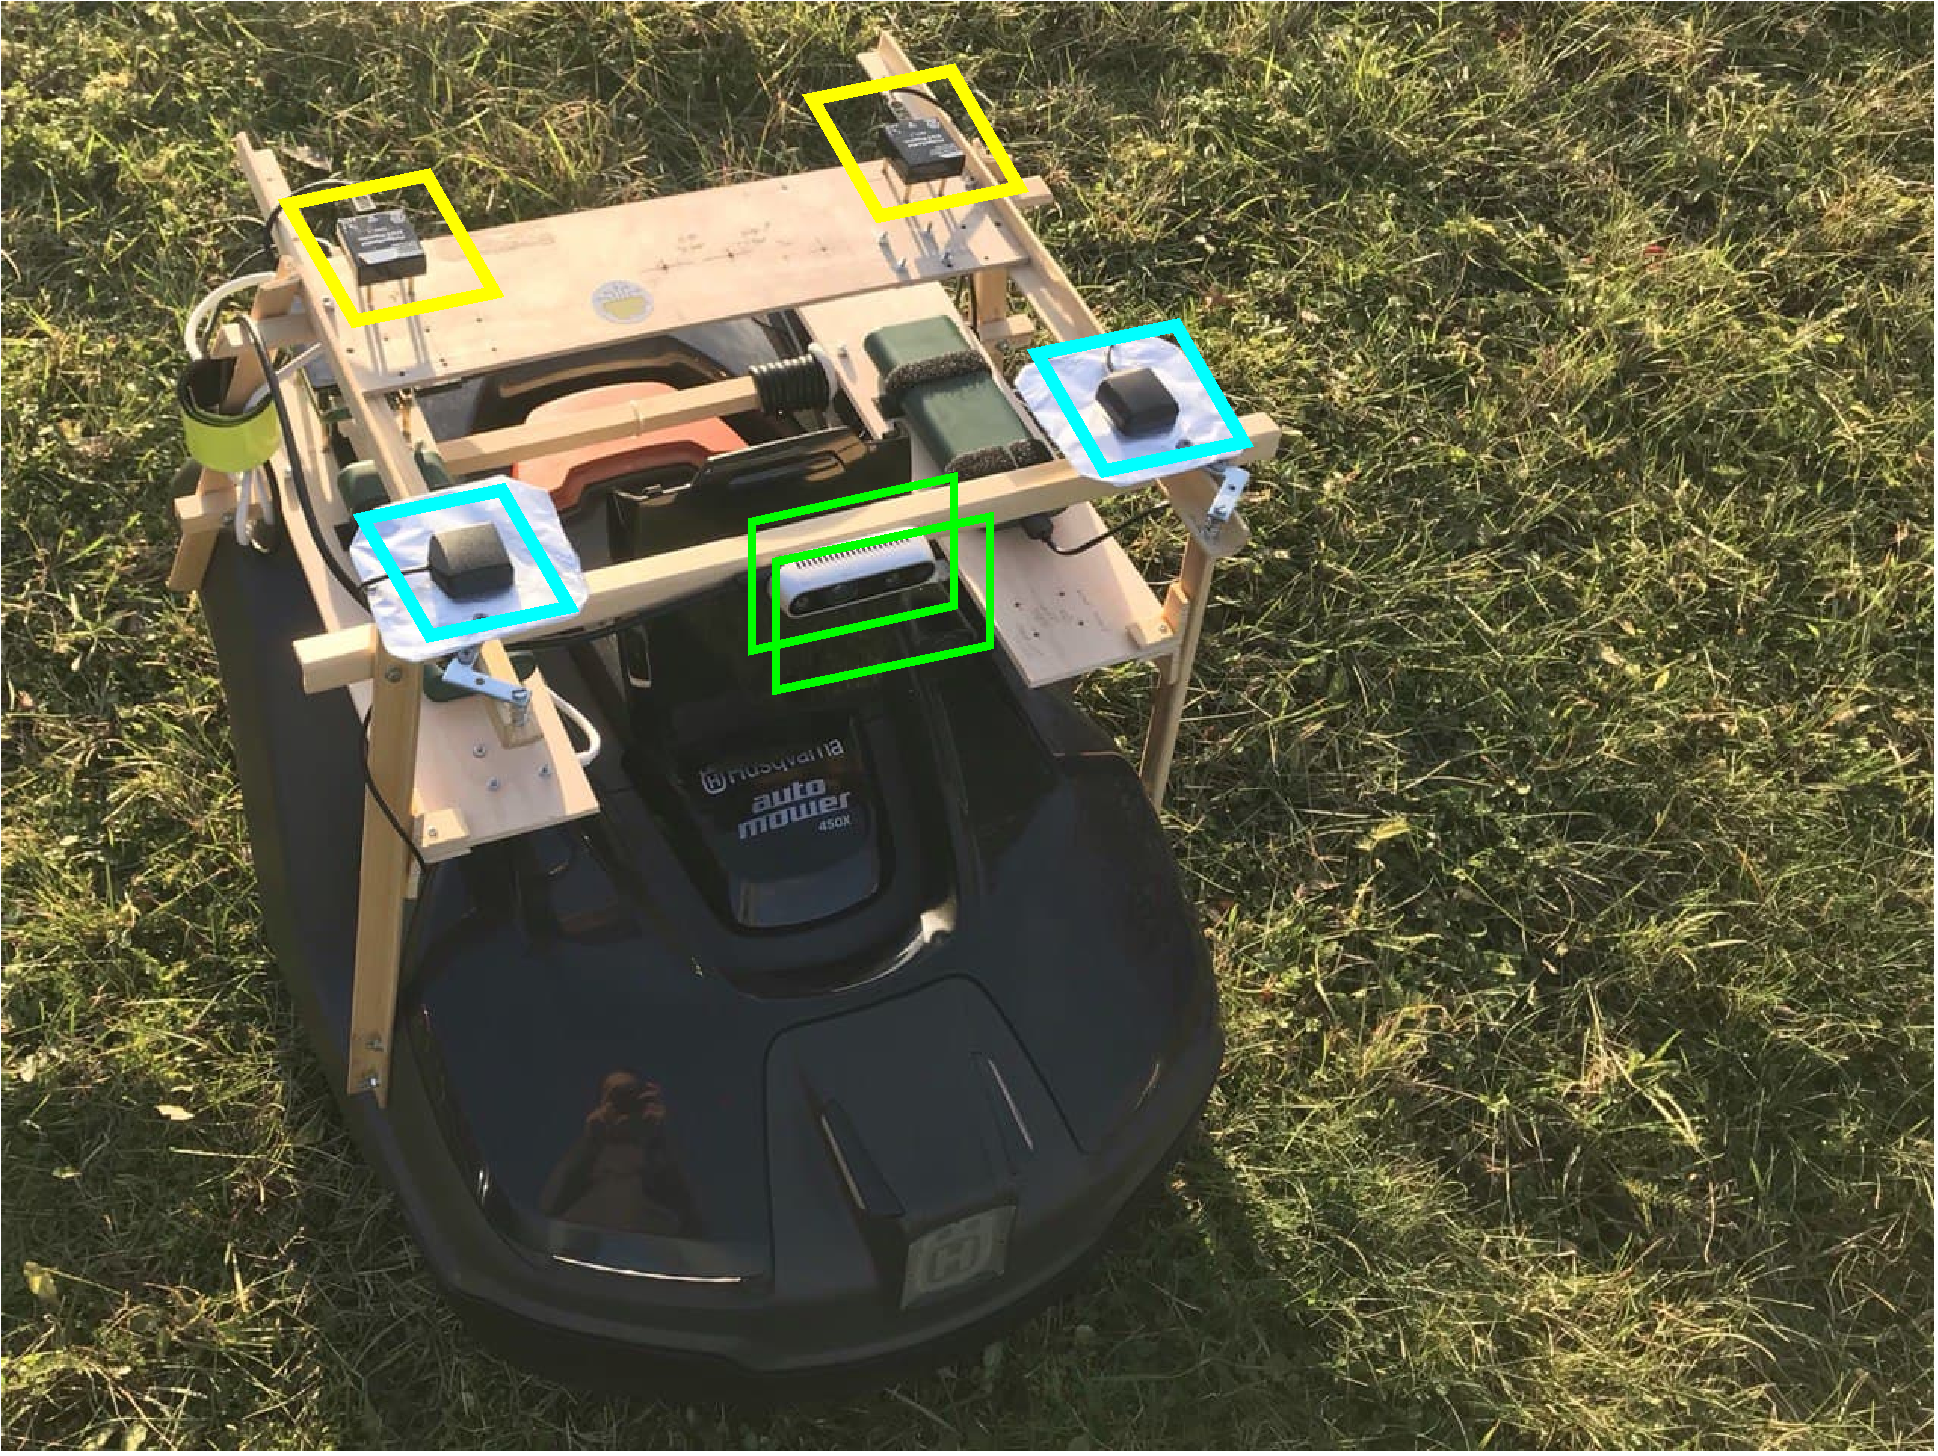
\includegraphics[width=1.0\textwidth]{Images/1-Introduction/projectTheme.pdf}
  \caption{Automower Model with focus on additional sensors}\label{fig:HardwareSetup}
  \end{center}
\end{figure}

\subsection{Considerations}
\com{
Describe the boundary/limits of your thesis project and what you are explicitly not going to do. This will help you bound your efforts – as you have clearly defined what is out of the scope of this thesis project. Explain the delimitations. These are all the things that could affect the study if they were examined and included in the degree project.
}

\noindent 
Since such \gls{ALM}s are consumer products, some constraints will be taken into account, such as the configuration complexity and the sensors cost analysis.
Some aspects regarding this degree project are described here:
\begin{itemize}
    \item The operation area is projected into a \Gls{2D} environment.
    \item The usage of an embedded device, such as a \gls{RPi}, limits the computational power of the module. Thus, the performance might not be as good as if a more powerful device would be used. %In this project, this aspect of optimization of the limited resources available on an embedded system will not be investigate.
    \item A complete \gls{SLAM} algorithm might be too computationally heavy to work with in a dynamic outdoor environment. 
    Instead, receiving directly a predefined map layout configuration of the environment with a given starting point of the automower should ease the process of mapping after localisation within it.
    \item Relying on a camera in outdoor settings means that the weather conditions and time of mowing can affect the results. 
    As such, the testing will be performed in similar configurations if possible, with an attitude towards limiting such a characteristic.
    \item A Range Finder Sensor was not considered as most of the outdoor environment will be sparse or empty.
    Thus, the sensor would not be able to provide valuable improvement to justify the expensive choice. 
    Moreover, such a sensor requires a relevant amount of computational power to be run.
\end{itemize}
They provide the rationale for the project to investigate some aspects more than others. 
Some of them are directly limiting and they are not be investigated for such a project.
Some others instead are part of the future works discussed at the end of this thesis


\section{Structure of the thesis}
\noindent In the following chapters the topics of this thesis are discussed as follows.

Chapter~\ref{ch:introduction}, Introduction, presents the problem and how its solution presented in the thesis will be evaluated.
The chapter also describes related work about similar approaches to general sensor fusion, about improvements to automower performances, and also provides an overview about competitors' approaches for the same task. 

Chapter~\ref{ch:background}, Background, presents relevant background information about mobile robots, localisation, mapping, and related works.

Chapter~\ref{ch:whatYouDid}, Methods, presents the methodologies and methods used to solve the problem. It also motivates and elaborates the implementation of the hardware and software .

Chapter~\ref{ch:resultsAndAnalysis}, Results, reveals and analyses the results obtained from varied methods through multiple experiments.

Chapter~\ref{ch:conclusion}, Conclusions, interprets and explains the results, wrapping up the thesis, and discussing what should be or can be done afterwards.


\cleardoublepage
%\clearpage
